\chapter{Background}
\section{Neural networks}
Ever since the invention of computer systems, it has always been a goal of scientists and engineers to create \gls{ai}. Current state of the art approaches are mimicking the human brain, more specifically the neurons inside the brain. Already in the fifties, Rosenblatt introduced his perceptron \cite{rosenblatt_perceptron_1958}. The perceptron is a single neuron able to learn linearly separable patterns. It does so by finding a hyperplane that separates the two classes. This hyperplane is called the decision surface or decision boundary. The concept of linear separability is explained in Figure \ref{fig:linear_separability} in two dimensions. \\

Unfortunately not all patterns are linearly separable. To overcome this problem, the neurons can be layered, creating an \gls{ann} in the process. Layering neurons sequentially is essentially a linear combination of neurons. This in itself does not create non-linear decision surfaces. Non-linear activation functions are added for the \gls{ann} to be able to learn more complex decision boundaries. Some commonly used activation functions are \gls{relu} \cite{relu}, Heaviside step function and softmax (or sigmoid when used on scalars). In Figure \ref{fig:activation_functions} the plots of the activation functions can be found. 



\begin{figure}
\tikzset{every picture/.style={line width=0.75pt}} %set default line width to 0.75pt        
\centering
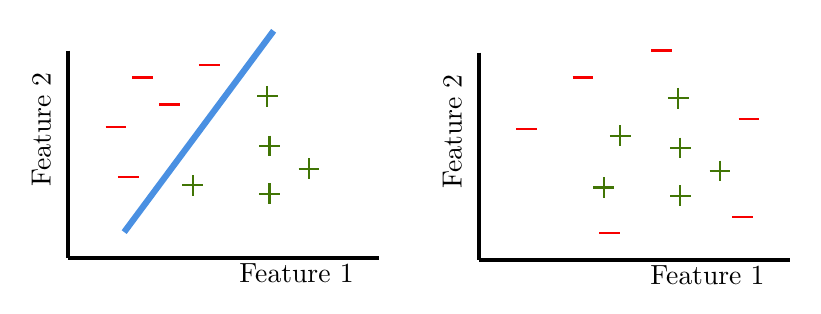
\begin{tikzpicture}[x=0.75pt,y=0.75pt,yscale=-1,xscale=1]
%uncomment if require: \path (0,300); %set diagram left start at 0, and has height of 300

%Straight Lines [id:da34928766651876697] 
\draw [line width=1.5]    (40,220) -- (190,220) ;
%Straight Lines [id:da5068123062544778] 
\draw [line width=1.5]    (40,120) -- (40,220) ;
%Straight Lines [id:da02959929373017789] 
\draw [color={rgb, 255:red, 247; green, 0; blue, 0 }  ,draw opacity=1 ]   (71,133) -- (81,133) ;
%Straight Lines [id:da023175201693992564] 
\draw [color={rgb, 255:red, 65; green, 117; blue, 5 }  ,draw opacity=1 ]   (132,166) -- (142,166) ;
%Straight Lines [id:da12599178724449778] 
\draw [color={rgb, 255:red, 65; green, 117; blue, 5 }  ,draw opacity=1 ]   (137,161) -- (137,171) ;

%Straight Lines [id:da014209875608111044] 
\draw [color={rgb, 255:red, 65; green, 117; blue, 5 }  ,draw opacity=1 ]   (95,185) -- (105,185) ;
%Straight Lines [id:da8046955093022794] 
\draw [color={rgb, 255:red, 65; green, 117; blue, 5 }  ,draw opacity=1 ]   (100,180) -- (100,190) ;

%Straight Lines [id:da8257858393303268] 
\draw [color={rgb, 255:red, 65; green, 117; blue, 5 }  ,draw opacity=1 ]   (151,177) -- (161,177) ;
%Straight Lines [id:da9904899777355851] 
\draw [color={rgb, 255:red, 65; green, 117; blue, 5 }  ,draw opacity=1 ]   (156,172) -- (156,182) ;

%Straight Lines [id:da4558392192767111] 
\draw [color={rgb, 255:red, 65; green, 117; blue, 5 }  ,draw opacity=1 ]   (132,189) -- (142,189) ;
%Straight Lines [id:da6277106773918533] 
\draw [color={rgb, 255:red, 65; green, 117; blue, 5 }  ,draw opacity=1 ]   (137,184) -- (137,194) ;

%Straight Lines [id:da6088809310233947] 
\draw [color={rgb, 255:red, 65; green, 117; blue, 5 }  ,draw opacity=1 ]   (131,142) -- (141,142) ;
%Straight Lines [id:da9717175839575936] 
\draw [color={rgb, 255:red, 65; green, 117; blue, 5 }  ,draw opacity=1 ]   (136,137) -- (136,147) ;

%Straight Lines [id:da05579332834233042] 
\draw [color={rgb, 255:red, 247; green, 0; blue, 0 }  ,draw opacity=1 ]   (84,146) -- (94,146) ;
%Straight Lines [id:da9339907902154778] 
\draw [color={rgb, 255:red, 247; green, 0; blue, 0 }  ,draw opacity=1 ]   (64,181) -- (74,181) ;
%Straight Lines [id:da801343700133325] 
\draw [color={rgb, 255:red, 247; green, 0; blue, 0 }  ,draw opacity=1 ]   (103,127) -- (113,127) ;
%Straight Lines [id:da6207217857469742] 
\draw [color={rgb, 255:red, 247; green, 0; blue, 0 }  ,draw opacity=1 ]   (58,157) -- (68,157) ;

%Straight Lines [id:da9774802467048496] 
\draw [line width=1.5]    (238,221) -- (388,221) ;
%Straight Lines [id:da8926029470752344] 
\draw [line width=1.5]    (238,121) -- (238,221) ;
%Straight Lines [id:da391932663930169] 
\draw [color={rgb, 255:red, 247; green, 0; blue, 0 }  ,draw opacity=1 ]   (360,200) -- (370,200) ;
%Straight Lines [id:da45698367355392255] 
\draw [color={rgb, 255:red, 65; green, 117; blue, 5 }  ,draw opacity=1 ]   (330,167) -- (340,167) ;
%Straight Lines [id:da8509197980874896] 
\draw [color={rgb, 255:red, 65; green, 117; blue, 5 }  ,draw opacity=1 ]   (335,162) -- (335,172) ;

%Straight Lines [id:da46487388742354385] 
\draw [color={rgb, 255:red, 65; green, 117; blue, 5 }  ,draw opacity=1 ]   (293,186) -- (303,186) ;
%Straight Lines [id:da6402947556346299] 
\draw [color={rgb, 255:red, 65; green, 117; blue, 5 }  ,draw opacity=1 ]   (298,181) -- (298,191) ;

%Straight Lines [id:da371430190479477] 
\draw [color={rgb, 255:red, 65; green, 117; blue, 5 }  ,draw opacity=1 ]   (349,178) -- (359,178) ;
%Straight Lines [id:da029152498087926304] 
\draw [color={rgb, 255:red, 65; green, 117; blue, 5 }  ,draw opacity=1 ]   (354,173) -- (354,183) ;

%Straight Lines [id:da7641303373625803] 
\draw [color={rgb, 255:red, 65; green, 117; blue, 5 }  ,draw opacity=1 ]   (330,190) -- (340,190) ;
%Straight Lines [id:da8503441823041022] 
\draw [color={rgb, 255:red, 65; green, 117; blue, 5 }  ,draw opacity=1 ]   (335,185) -- (335,195) ;

%Straight Lines [id:da14090483844456858] 
\draw [color={rgb, 255:red, 65; green, 117; blue, 5 }  ,draw opacity=1 ]   (329,143) -- (339,143) ;
%Straight Lines [id:da10211881619757635] 
\draw [color={rgb, 255:red, 65; green, 117; blue, 5 }  ,draw opacity=1 ]   (334,138) -- (334,148) ;

%Straight Lines [id:da8074255152632699] 
\draw [color={rgb, 255:red, 247; green, 0; blue, 0 }  ,draw opacity=1 ]   (296,208) -- (306,208) ;
%Straight Lines [id:da01705778265856206] 
\draw [color={rgb, 255:red, 247; green, 0; blue, 0 }  ,draw opacity=1 ]   (363,153) -- (373,153) ;
%Straight Lines [id:da4845113413868791] 
\draw [color={rgb, 255:red, 247; green, 0; blue, 0 }  ,draw opacity=1 ]   (283,133) -- (293,133) ;
%Straight Lines [id:da861487465385409] 
\draw [color={rgb, 255:red, 247; green, 0; blue, 0 }  ,draw opacity=1 ]   (256,158) -- (266,158) ;
%Straight Lines [id:da9913185077125697] 
\draw [color={rgb, 255:red, 247; green, 0; blue, 0 }  ,draw opacity=1 ]   (321,120) -- (331,120) ;
%Straight Lines [id:da016655837516902583] 
\draw [color={rgb, 255:red, 65; green, 117; blue, 5 }  ,draw opacity=1 ]   (301,161) -- (311,161) ;
%Straight Lines [id:da48554389877316395] 
\draw [color={rgb, 255:red, 65; green, 117; blue, 5 }  ,draw opacity=1 ]   (306,156) -- (306,166) ;


%Straight Lines [id:da7796305041163321] 
\draw [color={rgb, 255:red, 74; green, 144; blue, 226 }  ,draw opacity=1 ][line width=2.25]    (139,110.5) -- (67,207.5) ;

% Text Node
\draw (319,222) node [anchor=north west][inner sep=0.75pt]   [align=left] {Feature 1};
% Text Node
\draw (219,188) node [anchor=north west][inner sep=0.75pt]  [rotate=-270] [align=left] {Feature 2};
% Text Node
\draw (121,221) node [anchor=north west][inner sep=0.75pt]   [align=left] {Feature 1};
% Text Node
\draw (21,187) node [anchor=north west][inner sep=0.75pt]  [rotate=-270] [align=left] {Feature 2};


\end{tikzpicture}
\caption[Linear separability]{Linearly separable classes on the left and non-linearly separable classes on the right. Two classes are linearly separable if there exists a hyperplane for which all examples of one class are on the same side of this hyperplane, whilst all examples of the other class are on the other side of the hyperplane. In two dimensions, the hyperplane is a straight line.}
\label{fig:linear_separability}
\end{figure}

\begin{figure}
\centering
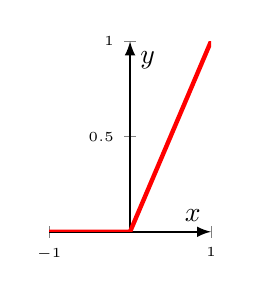
\begin{tikzpicture}
\begin{axis}[width=0.30\textwidth,
height=4cm,
axis lines=middle,
xlabel=$x$,
ylabel=$y$,
xmin=-1,
xmax=1,
ymin=0,
ymax=1,
xtick={-1,1},
ytick={0,0.5,1},
axis line style={-latex},
ticklabel style={font=\tiny,fill=white},
]
\addplot[ultra thick, color=red]{max(0,x)};
\end{axis}
\end{tikzpicture}
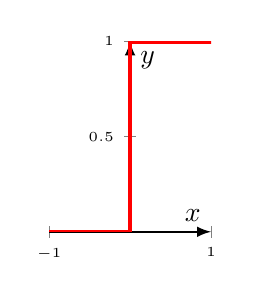
\begin{tikzpicture}
\begin{axis}[width=0.30\textwidth,
height=4cm,
axis lines=middle,
xlabel=$x$,
ylabel=$y$,
xmin=-1,
xmax=1,
ymin=0,
ymax=1,
xtick={-1,1},
ytick={0,0.5,1},
axis line style={-latex},
ticklabel style={font=\tiny,fill=white},
]
\addplot+[const plot, no marks, ultra thick, color=red] coordinates {(-10,0) (0,1) (10, 1)};
\end{axis}
\end{tikzpicture}
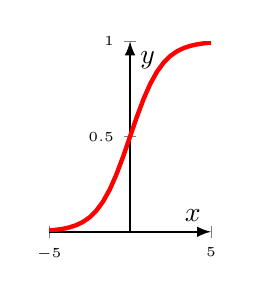
\begin{tikzpicture}
\begin{axis}[width=0.30\textwidth,
height=4cm,
axis lines=middle,
xlabel=$x$,
ylabel=$y$,
xmin=-5,
xmax=5,
ymin=0,
ymax=1,
xtick={-5,5},
ytick={0,0.5,1},
axis line style={-latex},
ticklabel style={font=\tiny,fill=white},
]
\addplot[ultra thick, color=red]{exp(x) / (1 + exp(x))};
\end{axis}
\end{tikzpicture}
\caption[Activiation functions]{Plots of different activation functions. From left to right: \gls{relu}, Heaviside step and sigmoid.}
\label{fig:activation_functions}
\end{figure}


\section{Adversarial attacks}

\section{Particle swarm optimization}



